\chapter{ROS 2 Middleware Implementation for WebAssembly}

    The design of a custom middleware implementation, \textsf{rms\_wasm}, that can be cross-compiled to WebAssembly modules is divided into three distinct packages as observed in Figure~\ref{fig:rmwwasm}.

    \begin{figure}[htbp]
        \centering
        \vspace{1em}
        \begin{tikzpicture}
            \node (pkg) [
                rectangle,
                rounded corners,
                draw = textColor,
                fill = igmrLightBlue!10!bgColor,
                text height = 7cm,
                align = justify,
                minimum width = 14cm,
                text width = 13.5cm,
            ] {\textsf{rmw\_wasm}};

            \node (rwc) [
                packBox,
                yshift = 2.5cm,
                fill = igmrLightBlue!30!bgColor,
                ] {\textsf{rmw\_wasm\_cpp}};

            \node (wcpp) [
                packBox,
                yshift = 0.5cm,
                fill = igmrLightBlue!30!bgColor,
                ] {\textsf{wasm\_cpp}};

            \node (wjs) [
                packBox,
                yshift = -2.5cm,
                fill = igmrLightBlue!30!bgColor,
                ] {\textsf{wasm\_js}};
            
            \node (ems) [
                rectangle,
                yshift = -1cm,
                xshift = 1.5cm,
                ] {\textsf{emscripten::val}};

            \draw[thick] (rwc) -- (wcpp);
            \draw[thick] (wcpp) -- (wjs);

        \end{tikzpicture}
        \vspace{1em}
        \caption{Architecture of custom middleware implementation to target WebAssembly.}
        \label{fig:rmwwasm}
    \end{figure}

    \section{\textsf{rmw\_wasm\_cpp}}

        The first package, \textsf{rmw\_wasm\_cpp}, works as the ``adapter'' between \ac{ROS} 2 and the designed middleware. This package implements all of the functions required for \textsf{rmw} as described in Section~\ref{ssec:minimal}. The source code for this package is entirely written in C++ and can be found: TODO:

        TODO: add diagram

    \section{\textsf{wasm\_cpp}}

        The role of \textsf{wasm\_cpp} is to TODO: and to function as a bridge to JavaScript functions.
    \section{\textsf{wasm\_js}}


    \begin{figure}[htbp]
        \centering
        \begin{tikzpicture}%[show background grid]
            \begin{abstractclass}[text width=5cm]{Participant}{0,0}
                \attribute{- name : String}
                \attribute{- role : String}
                \attribute{- gid  : String}

                \operation{- is\_valid\_name()}
                \operation{- is\_valid\_role()}
                \operation{- registration()}
                \operation{- deregistration()}
            \end{abstractclass}

            \begin{class}[text width=5cm]{Publisher}{-5,-6}
                \inherit{Participant}
                \attribute{- name = topic\_name}
                \attribute{- role = publisher}
                \operation{+ publish(message : String)}
            \end{class}

            \begin{class}[text width=5cm]{Subscriber}{5,-6}
                \inherit{Participant}
                \attribute{- name = topic\_name}
                \attribute{- role = subscriber}
                \operation{+ get\_message() : String}
            \end{class}

            \begin{class}[text width=6.5cm]{ServiceServer}{-4,-11}
                \inherit{Participant}
                \attribute{- name = service\_name}
                \attribute{- role = service\_server}
                \operation{+ take\_request() : String}
                \operation{+ send\_response(response : String)}
            \end{class}

            \composition{ServiceServer}{}{}{Publisher}
            \composition{ServiceServer}{}{}{Subscriber}

            \begin{class}[text width=6.5cm]{ServiceClient}{4,-11}
                \inherit{Participant}
                \attribute{- name = service\_name}
                \attribute{- role = service\_client}
                \operation{+ send\_request(request : String)}
                \operation{+ take\_response() : String}
                \operation{+ is\_service\_available() : Bool}
            \end{class}

            \composition{ServiceClient}{}{}{Publisher}
            \composition{ServiceClient}{}{}{Subscriber}

        \end{tikzpicture}
        \caption{A class diagram}
    \end{figure}
    


\section{Design of Web Elements}

\section{Web Workers}

    

\section{Message Stacks}

    \begin{figure}[htbp]
        \centering
        \begin{subfigure}[t]{0.32\textwidth}
            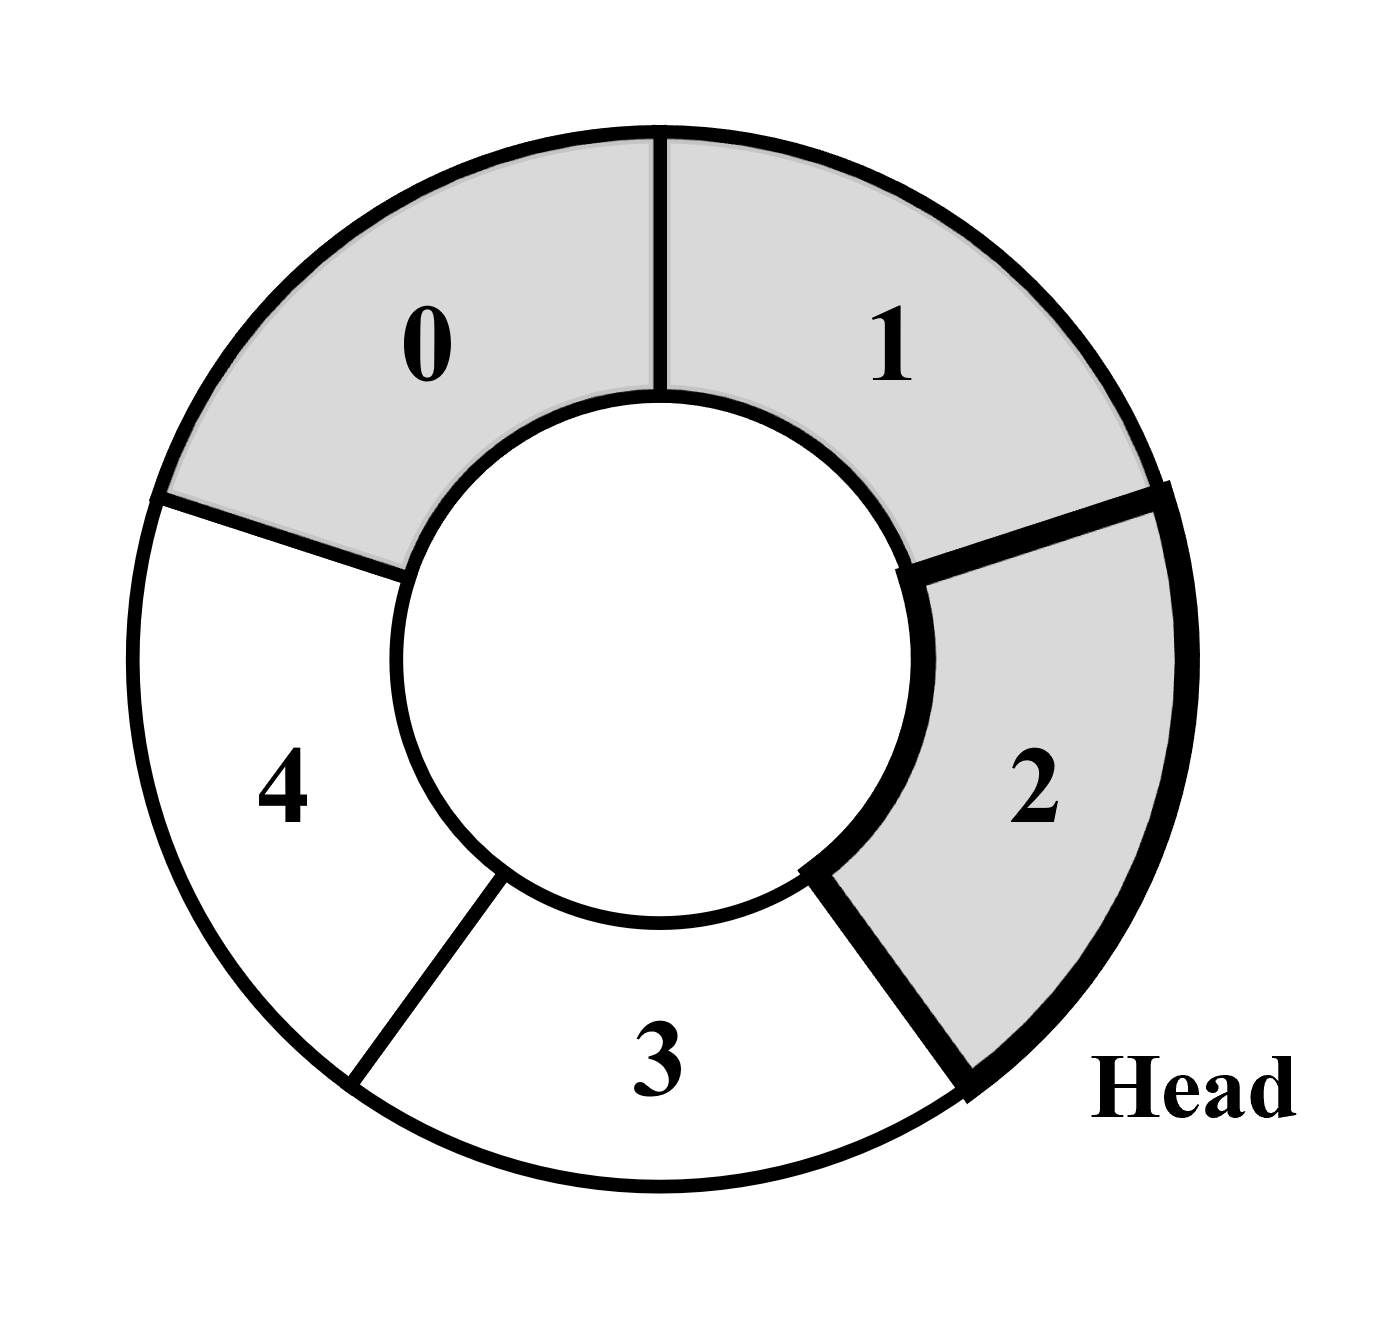
\includegraphics[height=0.9\textwidth]{07_stack0.png}
            \caption{Filling stack}
        \end{subfigure}
        \begin{subfigure}[t]{0.32\textwidth}
            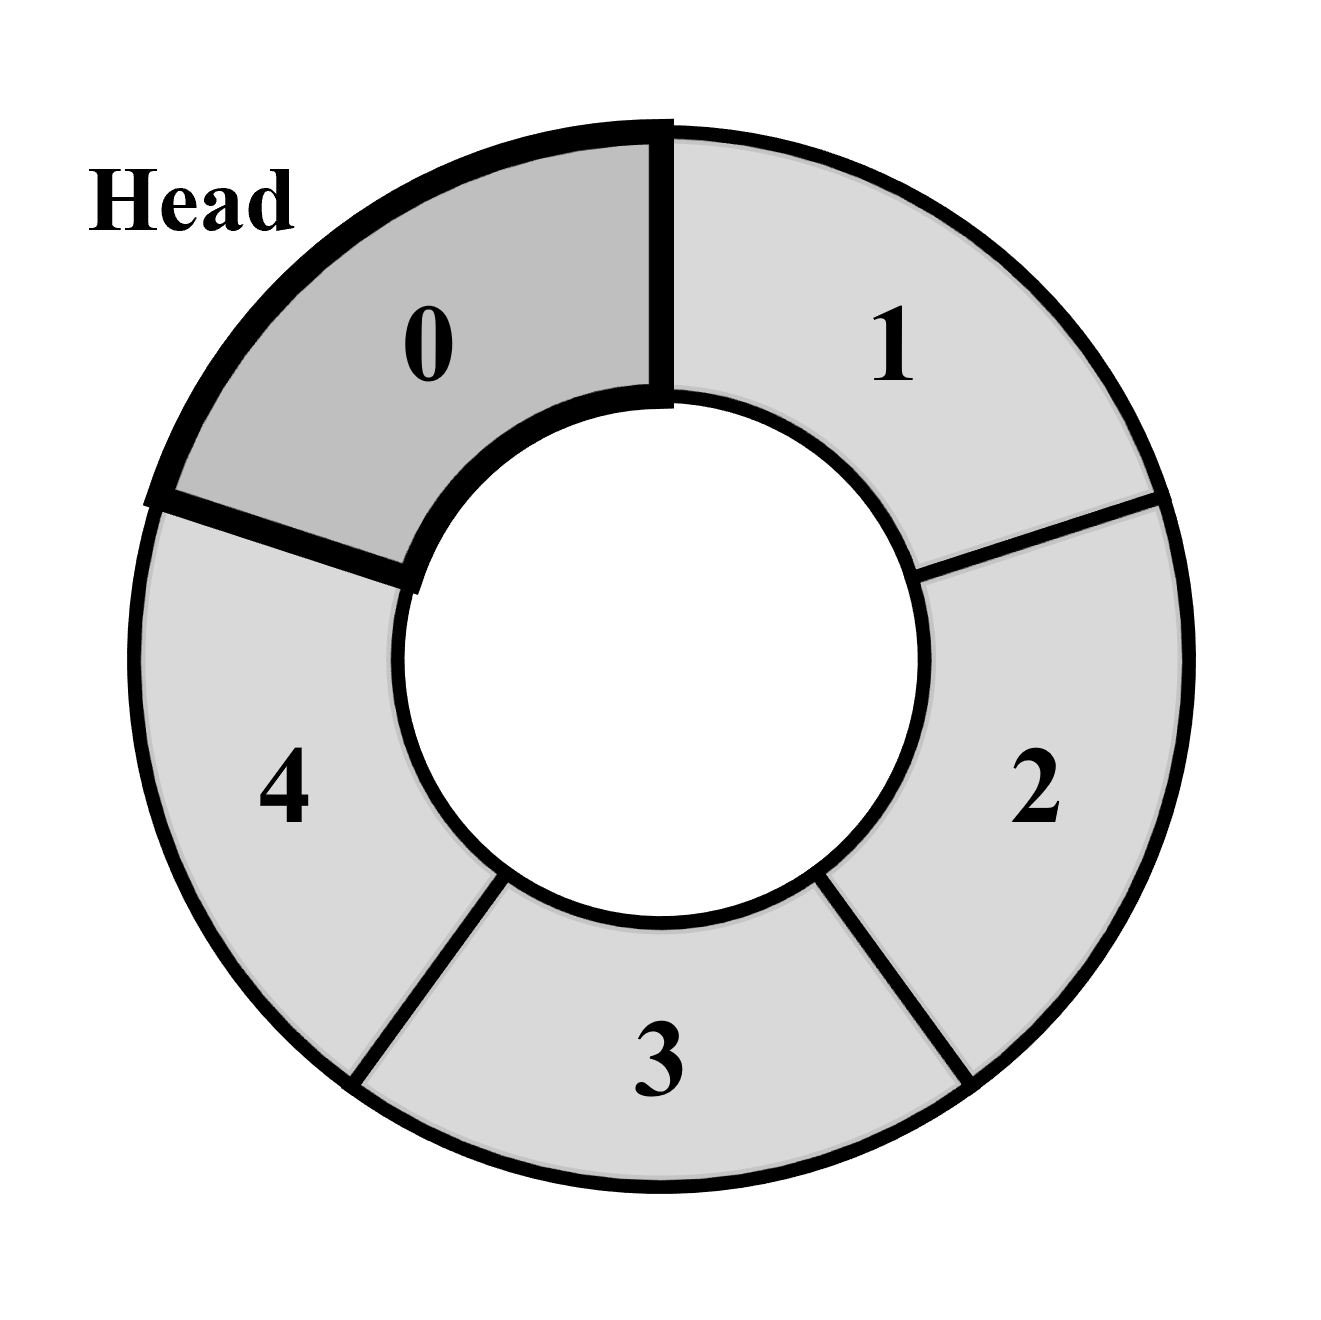
\includegraphics[height=0.9\textwidth]{07_stack1.png}
            \caption{Overwriting stack}
        \end{subfigure}
        \begin{subfigure}[t]{0.32\textwidth}
            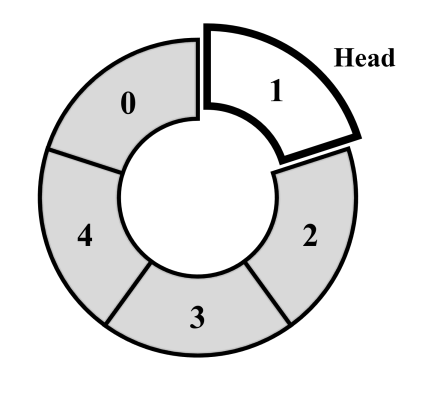
\includegraphics[height=0.9\textwidth]{07_stack2.png}
            \caption{Reading stack}
        \end{subfigure}
        \caption{Modified Circular Stack, \ac{LIFO}}\label{fig:circleStack}
    \end{figure}

- Web workers, what are they? why are they needed?
- Communication channels
- Registry of topics/subs/pubs
- Message handling
width